%
%Не забыть:
%--------------------------------------
%Вставить колонтитулы, поменять название на титульнике



%--------------------------------------

\documentclass[a4paper, 12pt]{article} 

%--------------------------------------
%Russian-specific packages
%--------------------------------------
%\usepackage[warn]{mathtext}
\usepackage[T2A]{fontenc}
\usepackage[utf8]{inputenc}
\usepackage[english,russian]{babel}
\usepackage[intlimits]{amsmath}
\usepackage{esint}
%--------------------------------------
%Hyphenation rules
%--------------------------------------
\usepackage{hyphenat}
\hyphenation{ма-те-ма-ти-ка вос-ста-нав-ли-вать}
%--------------------------------------
%Packages
%--------------------------------------
\usepackage{amsmath}
\usepackage{amssymb}
\usepackage{amsfonts}
\usepackage{amsthm}
\usepackage{latexsym}
\usepackage{mathtools}
\usepackage{etoolbox}%Булевые операторы
\usepackage{extsizes}%Выставление произвольного шрифта в \documentclass
\usepackage{geometry}%Разметка листа
\usepackage{indentfirst}
\usepackage{wrapfig}%Создание обтекаемых текстом объектов
\usepackage{fancyhdr}%Создание колонтитулов
\usepackage{setspace}%Настройка интерлиньяжа
\usepackage{lastpage}%Вывод номера последней страницы в документе, \lastpage
\usepackage{soul}%Изменение параметров начертания
\usepackage{hyperref}%Две строчки с настройкой гиперссылок внутри получаеммого
\usepackage[usenames,dvipsnames,svgnames,table,rgb]{xcolor}% pdf-документа
\usepackage{multicol}%Позволяет писать текст в несколько колонок
\usepackage{cite}%Работа с библиографией
\usepackage{tikz}%Рисование рисунков
% Для картинок Моти
\usepackage{misccorr}
\usepackage{lscape}
\usepackage{cmap}


\usepackage{graphicx,xcolor}
\graphicspath{{Pictures/}}
\DeclareGraphicsExtensions{.pdf,.png,.jpg}

%----------------------------------------
%Список окружений
%----------------------------------------
\newenvironment {theor}[2]
{\smallskip \par \textbf{#1.} \textit{#2}  \par $\blacktriangleleft$}
{\flushright{$\blacktriangleright$} \medskip \par} %лемма/теорема с доказательством
\newenvironment {proofn}
{\par $\blacktriangleleft$}
{$\blacktriangleright$ \par} %доказательство
%----------------------------------------
%Список команд
%----------------------------------------
\newcommand{\grad}
{\mathop{\mathrm{grad}}\nolimits} %градиент

\newcommand{\diver}
{\mathop{\mathrm{div}}\nolimits} %дивергенция

\newcommand{\Def}[1]
{\underline{\textbf{#1}}} %определение

\newcommand{\RN}[1]
{\MakeUppercase{\romannumeral #1}} %римские цифры

\newcommand {\theornp}[2]
{\textbf{#1.} \textit{ #2} \par} %Написание леммы/теоремы без доказательства

\newcommand{\qrq}
{\ensuremath{\quad \Rightarrow \quad}} %Человеческий знак следствия

\newcommand{\qlrq}
{\ensuremath{\quad \Leftrightarrow \quad}} %Человеческий знак равносильности

\renewcommand{\phi}{\varphi} %Нормальный знак фи

\newcommand{\me}
{\ensuremath{\mathbb{E}}}

\newcommand{\md}
{\ensuremath{\mathbb{D}}}



%\renewcommand{\vec}{\overline}



%----------------------------------------
%Разметка листа
%----------------------------------------
\geometry{top = 3cm}
\geometry{bottom = 2cm}
\geometry{left = 1.5cm}
\geometry{right = 1.5cm}
%----------------------------------------
%Колонтитулы
%----------------------------------------
\pagestyle{fancy}%Создание колонтитулов
\fancyhead{}
%\fancyfoot{}
\fancyhead[R]{\textsc{Вводная лабораторная работа}}%Вставить колонтитул сюда
%----------------------------------------
%Интерлиньяж (расстояния между строчками)
%----------------------------------------
%\onehalfspacing -- интерлиньяж 1.5
%\doublespacing -- интерлиньяж 2
%----------------------------------------
%Настройка гиперссылок
%----------------------------------------
\hypersetup{				% Гиперссылки
	unicode=true,           % русские буквы в раздела PDF
	pdftitle={Заголовок},   % Заголовок
	pdfauthor={Автор},      % Автор
	pdfsubject={Тема},      % Тема
	pdfcreator={Создатель}, % Создатель
	pdfproducer={Производитель}, % Производитель
	pdfkeywords={keyword1} {key2} {key3}, % Ключевые слова
	colorlinks=true,       	% false: ссылки в рамках; true: цветные ссылки
	linkcolor=black,          % внутренние ссылки
	citecolor=green,        % на библиографию
	filecolor=magenta,      % на файлы
	urlcolor=cyan           % на URL
}
%----------------------------------------
%Работа с библиографией (как бич)
%----------------------------------------
%\renewcommand{\refname}{Список литературы}%Изменение названия списка литературы для article
%\renewcommand{\bibname}{Список литературы}%Изменение названия списка литературы для book и report
%----------------------------------------
\begin{document}
	\begin{titlepage}
		\begin{center}
			$$$$
			$$$$
			$$$$
			$$$$
			{\Large{НАЦИОНАЛЬНЫЙ ИССЛЕДОВАТЕЛЬСКИЙ УНИВЕРСИТЕТ}}\\
			\vspace{0.1cm}
			{\Large{ВЫСШАЯ ШКОЛА ЭКОНОМИКИ}}\\
			\vspace{0.25cm}
			{\large{Факультет физики}}\\
			\vspace{5.5cm}
			{\Huge\textbf{{Лабораторная работа}}}\\%Общее название
			\vspace{1cm}
			{\LARGE{<<Вводная лабораторная работа>>}}\\%Точное название
			\vspace{2cm}
			{Работу выполнил студент 2 курса}\\
			{Захаров Сергей Дмитриевич}
			\vfill
			
\includegraphics[width = 0.2\textwidth]{HSElogo}\\
			\vfill
			Москва\\
			2019
		\end{center}
	\end{titlepage}

\tableofcontents

\newpage

\section{Цели работы}

Перед началом выполнения работы были поставлены следующие цели:

\begin{enumerate}
	\item Определить индуктивность исследуемой катушки.
	
	\item Определить емкость исследуемого конденсатора.
	
	\item Получить ВАХ (вольт-амперную характеристику) диода.
\end{enumerate}

\section{Оборудование}

\begin{itemize}
	\item Цифровой осциллограф со встроенным генератором различных форм напряжения и два щупа для него
	
	\item Мультиметр и щупы для него
	
	\item Переменное сопротивление
	
	\item Катушка неизвестной индуктивности
	
	\item Конденсатор неизвестной емкости
	
	\item Макетная плата и соединительные провода
\end{itemize}

\section{Описание метода выполнения работы}

%Перед переходом к выполнению каждой из частей работы на переменном сопротивление было выставлено сопротивление \boxed{$R = 61.5$ \text{ Ом}}.

\subsection{Определение индуктивности катушки}

Чтобы определить индуктивность катушки можно воспользоваться довольно простым методом, основанным на фактом из векторных диаграмм, а именно следующим:

\begin{equation}
	\tg\Delta\phi = \frac{\omega L}{R}
	\label{eq:phi_beg}
\end{equation}

Здесь $R$ --- активное сопротивление цепи, $L$ --- искомая индуктивность катушки, $\omega$ --- частота колебаний в контуре, $\Delta\phi$ --- разность фаз напряжений на катушке индуктивности и активном сопротивлении.

Таким образом мы получаем простую формулу для расчета:

\begin{equation}
	L = \frac{R \cdot \tg\Delta\phi}{\omega}
	\label{eq:L}
\end{equation}

\subsection{Определение емкости
	 конденсатора}

Для определения емкости конденсатора, в целом, можно было также воспользоваться способом, указанным выше, однако было решено разнообразить процесс и воспользоваться иным методом. Для этого была собрана схема, представленная на рисунке. %референс на схему
После этого с генератора осциллографа подавался сигнал в форме меандра (прямоугольный сигнал).

Получим формулу для емкости конденсатора. С одной стороны, ток в цепи можно выразить с помощью емкости конденсатора и напряжения на нем, с другой --- с помощью закона Ома для резистора (рассматриваем только тот участок времени, где конденсатор заряжается). Запишем:

\begin{equation}
	\label{C_diff}
	I = - C \frac{d U_c}{d t} = \frac{U - U_c}{R}
\end{equation}

Решив это дифференциальное уравнение, получим:

\begin{equation}
	\label{U_condencator}
	U = U\cdot(1 - e^{-t / (RC)})
\end{equation}

Чтобы теперь найти емкость конденсатора, достаточно посмотреть, за какое время $t_0$ он зарядится до напряжения $U_c = U \cdot (1 - 1 / e)$. В таком случае емкость выразится следующим образом:

\begin{equation}
	\label{C_final}
	\frac{t}{RC} = 1 \qrq C = \frac{t}{R}
\end{equation}

\section{Выполнение работы}

\subsection{Определение индуктивности катушки}

На основании формулы \ref{eq:L} мы можем с легкостью посчитать индуктивность катушки, приняв активное сопротивление цепи равным сопротивлению резистора $R = 4$ кОм. Данные представлены в форме графика на рисунке \ref{fig:inductivity}.

\begin{figure}[h!]
	\centering
	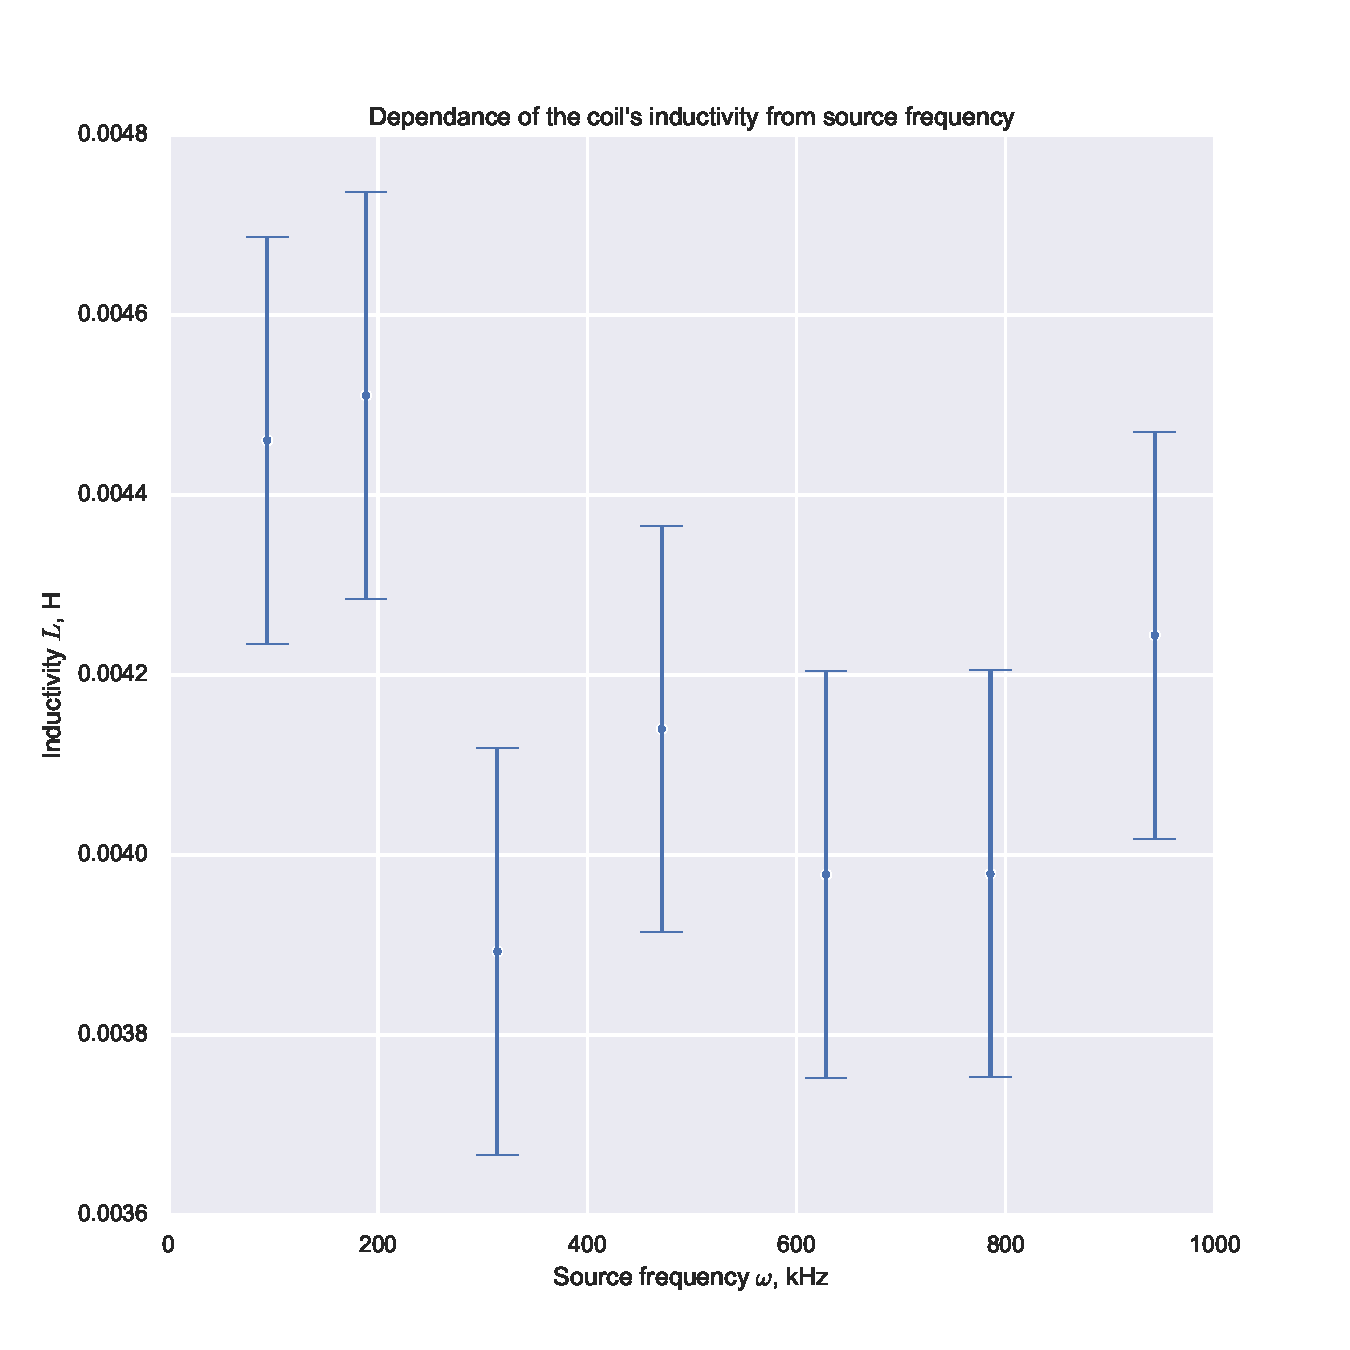
\includegraphics[width=\textwidth]{Inductivity.pdf}
	\caption{Зависимость индуктивности катушки от частоты колебаний в контуре}
	\label{fig:inductivity}
\end{figure}

Взяв среднюю индуктивность, получим, что она равна $\boxed{L = 0.00417 \text{ Гн} = 4.17 \text{ мГн}}$.

\subsection{Определение емкости конденсатора}

С помощью схемы, указанной на %ссылка
были получены данные, представленные на рисунке \ref{fig:capacitor}. При анализе данных получаем, что искомая доля напряжения накапливается за время $\boxed{t = 22.5\text{ нс}}$. Основываясь на полученной ранее формуле (\ref{C_final}), получаем, что искомая емкость конденсатора равна $\boxed{C = 0.36\text{ нФ}}$ приняв, что активное сопротивление цепи равно сопротивлению резистора $R = 62.5$ Ом.

\begin{figure}[h!]
	\center
	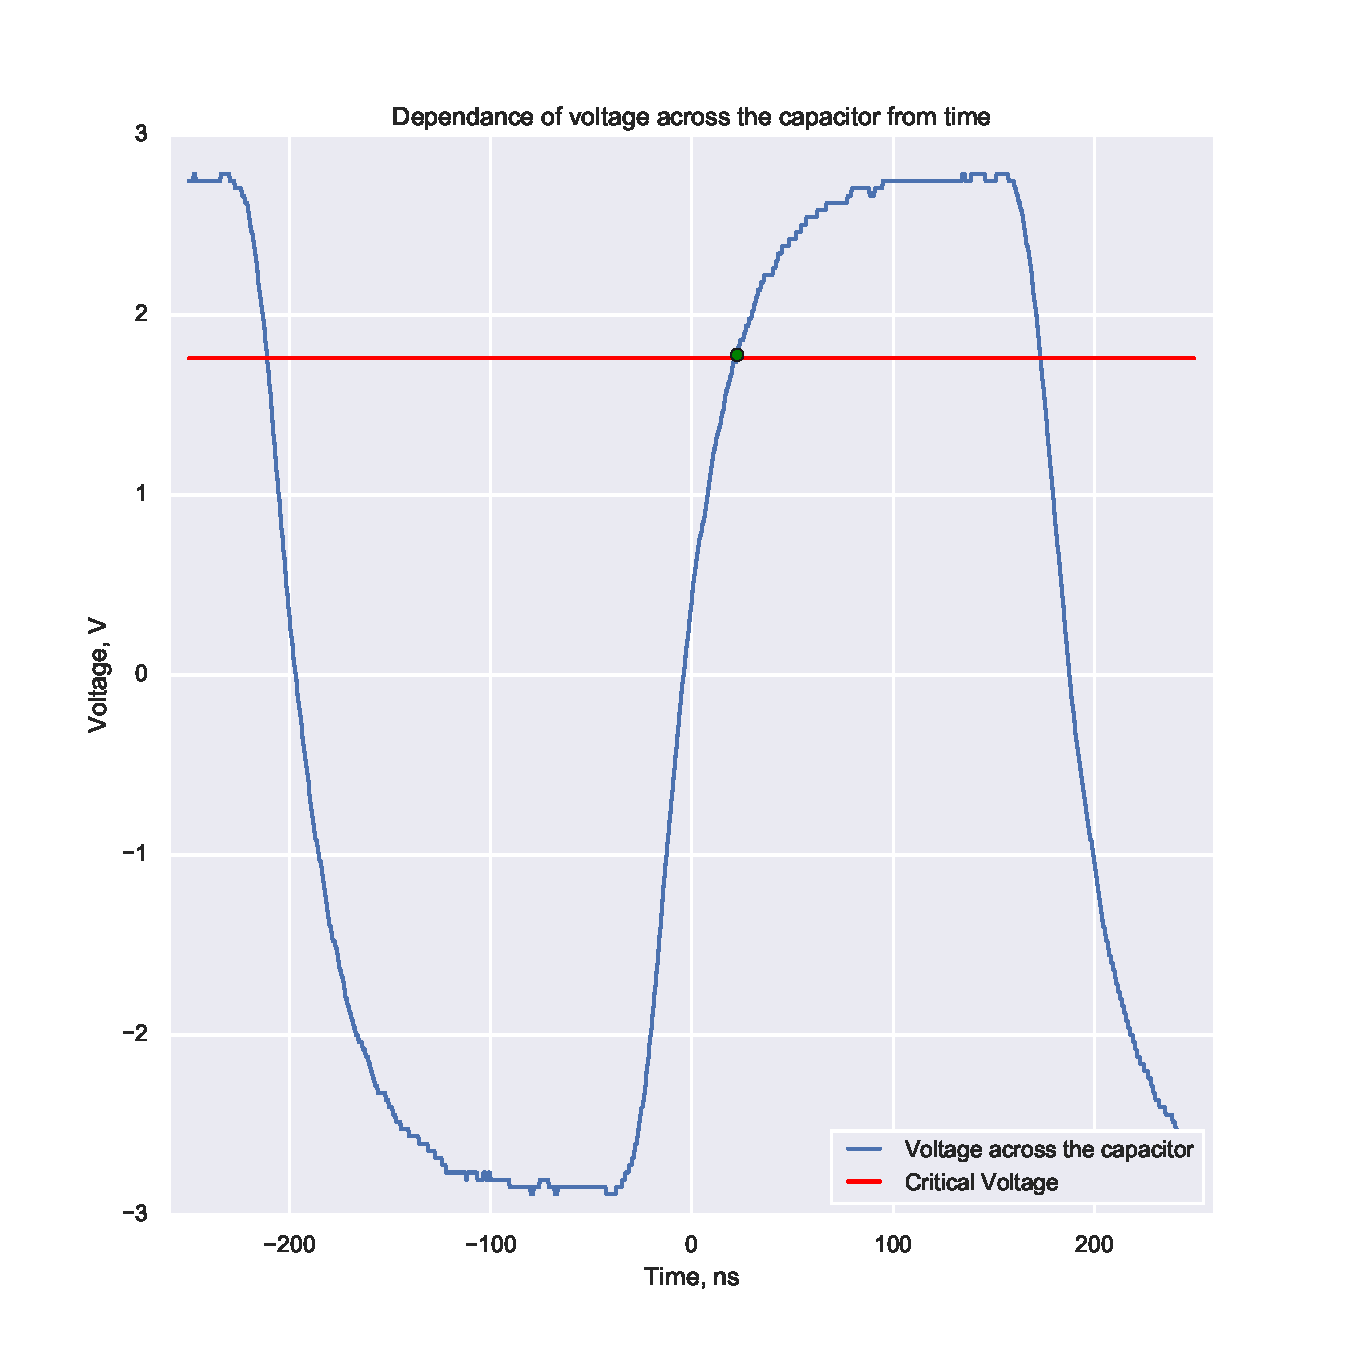
\includegraphics[width=0.9\linewidth]{Capacitor.pdf}
	\caption{Зависимость напряжения на конденсаторе от времени}
	\label{fig:capacitor}
\end{figure}

\subsection{Построение ВАХ диода}

ВАХ диода была получена переводом осциллографа в режим XY и представлена на рисунке~\ref{fig:vah}.

\begin{figure}[h!]
	\centering
	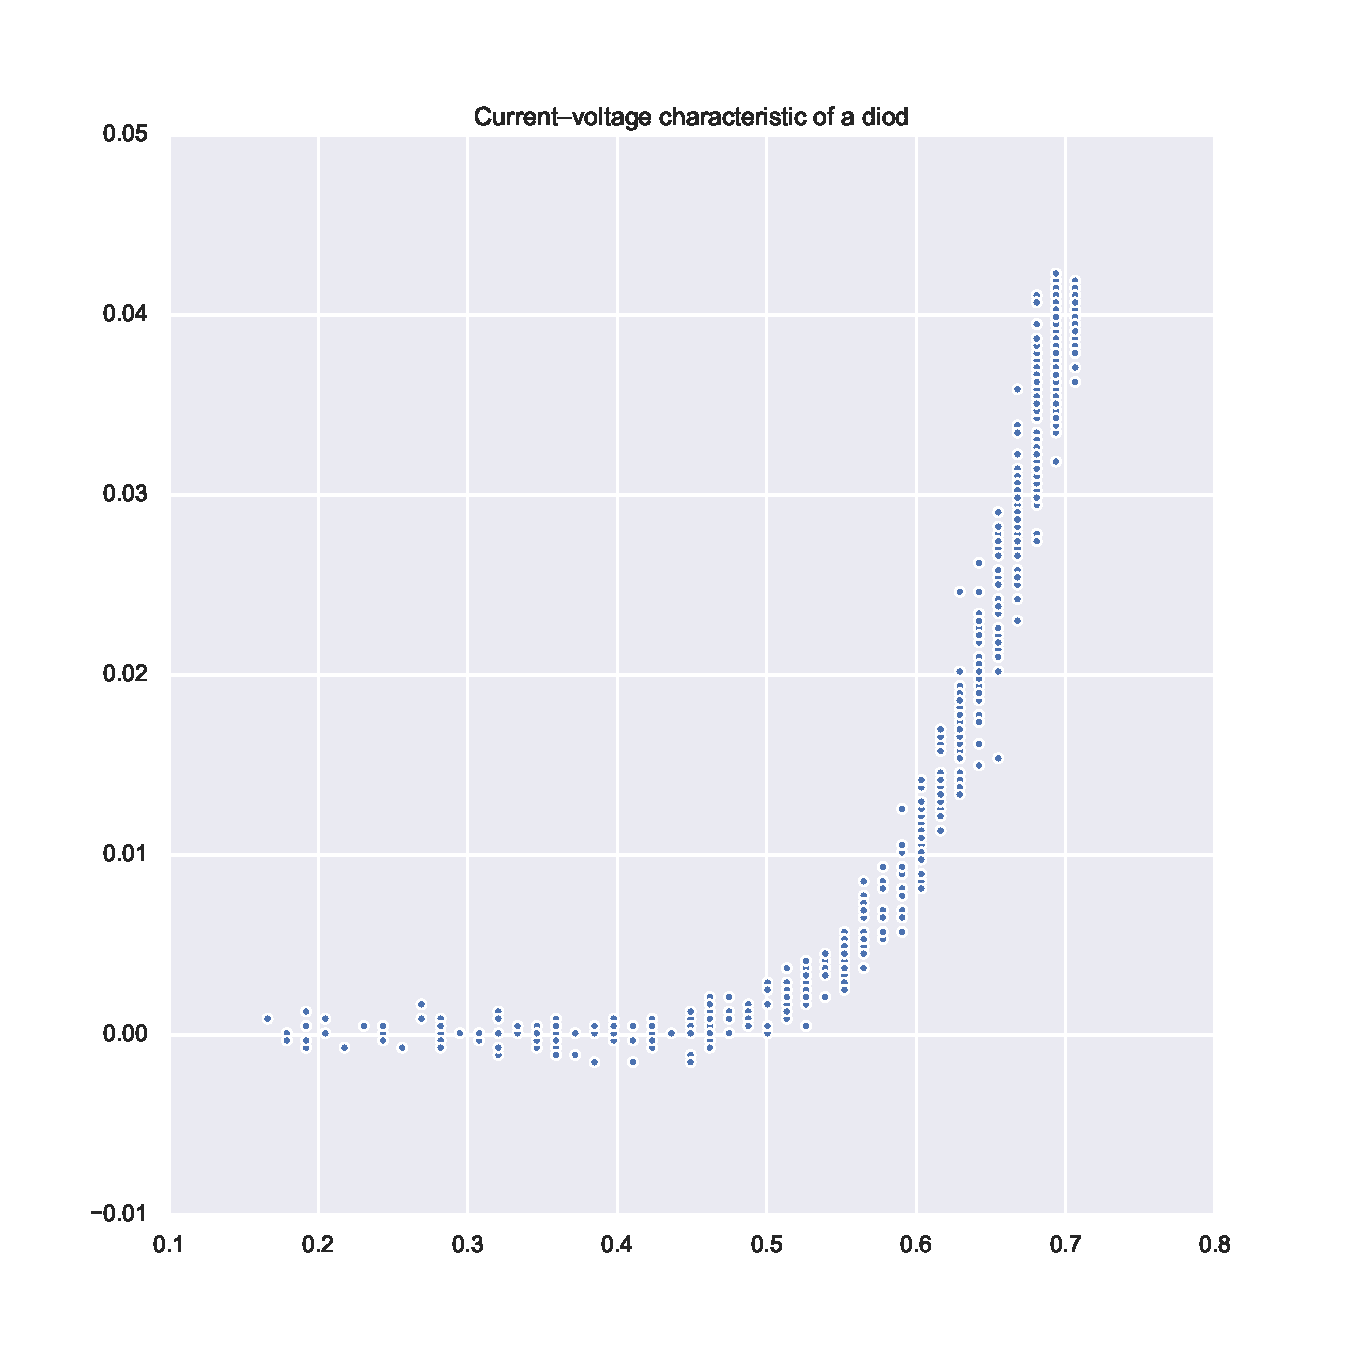
\includegraphics[width = \textwidth]{Vah.pdf}
	\caption{Вольт-амперная характеристика диода}
	\label{fig:vah}
\end{figure}








\end{document}





















